%\documentclass[tikz, border=5pt]{standalone}
\begin{document}
	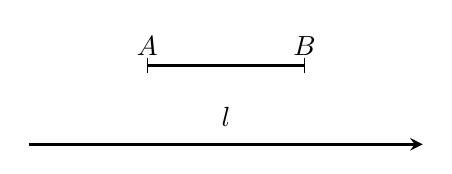
\begin{tikzpicture}

		% 绘制水平直线
		\draw[line width=1pt] (-1,1) -- (1,1);
		
		% 点A:标记文字、小竖线
		\node at (-1,1) [above] {$A$};
		\draw (-1,1.1) -- (-1,0.9);  % A点的垂直小竖线(上下各延伸0.1单位)
		
		% 点B:标记文字、小竖线
		\node at (1,1) [above] {$B$};
		\draw (1,1.1) -- (1,0.9);  % B点的垂直小竖线
		
		% 绘制射线,从原点(0,0)出发向右延伸5cm,右侧有三角形箭头
		\draw[->, >=stealth, line width=1pt] (-2.5,0) -- ++(5cm,0);
		% 在射线上方添加标签l
		\node[above] at (0cm, 0.1cm) {$l$};

	\end{tikzpicture}
\end{document}
